The discussion thus far has focused mainly on encoding logical states in the
entire 2D array of qubits that make up a particular surface. This is the
necessary experimental first step in proving the viability of surface codes, but
creating different 2D sheets for each logical qubit is not the most effective
way to scale up this scheme for multiple logicals. One key candidate approach
suggests encoding qubits using \textit{defects} in the lattice structure of the
surface code, by switching off certain parity measurements to define logical
qubits. We will now outline this procedure.

In order to encode a qubit in a surface code, it suffices to define two logical
operations, namely $Z_L$ and $X_L$, which fulfill the commutation relation
$[Z_L,X_L] = 2Z_LX_L$. When multiple qubits are required, the $X_L$ and $Z_L$
operations among different qubits must commute. Figure \ref{fig:surface_code}
shows one of the possible set of physical operations that can lead to the
required logical operations. In this case, a chain of Z (X) gates in the data
qubits, represented with the red (blue) line, are one of the multiple choices to
define a logical $Z_L$ ($X_L$) operation.

\begin{figure}[htbp]
  \centering
  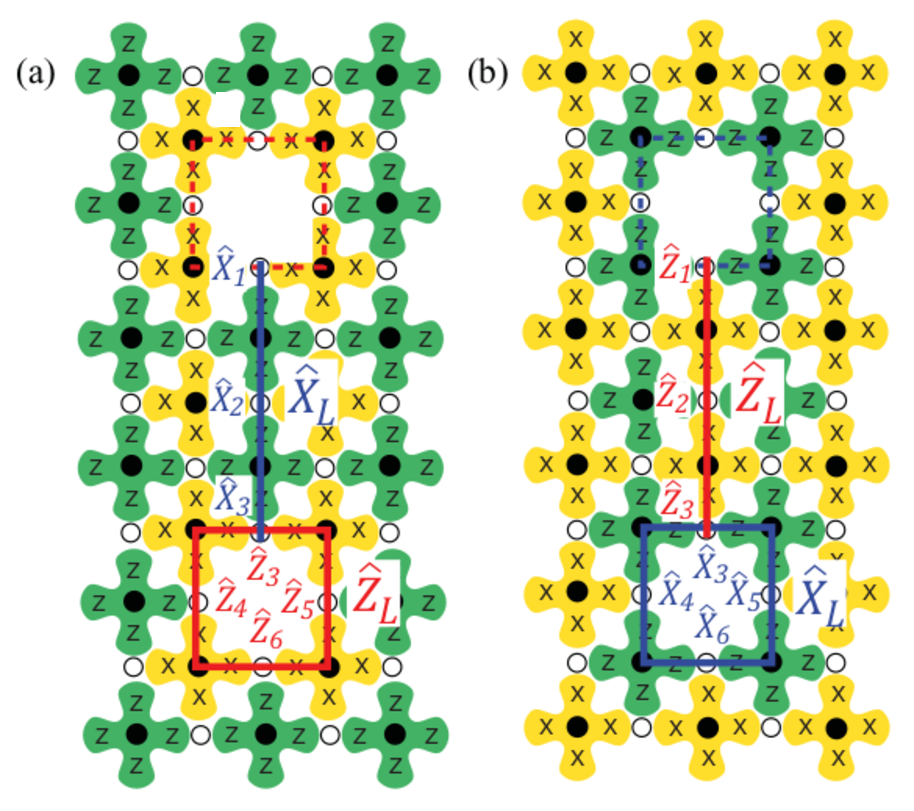
\includegraphics[width=0.5\textwidth]{images/surface_code_cuts.pdf}
  \caption{Examples of a Z-cut (a) and X-cut (b) qubit in a surface lattice. The
    logical gates are defined such that they satisfy the appropriate commutation
    relations. Moving defects further from each other can increase the code
    distance (the minimum number of gates required for a logical operation).}
  \label{fig:cuts}
\end{figure}

However, even though a set qubits may be fully defined in terms of these
operations, it is still necessary to perform arbitrary rotations and multi-qubit
gates on them. It is a well-known result of quantum computation that that it
suffices to be able to apply the standard H, T and CNOT gates to perform
universal computation \cite{nielsen_chuang_2010}. However, from the DiVincenzo
criteria \cite{DiCincenzoCriteria}, we see that initialization and
measurement capabilities are also necessary.

Although all these operations can be performed using one lattice per qubit,
it is much more efficient to use a defect based approach. In this case, a qubit
consists of two Z-cut (X-cut) defects, where, in its simplest form, two Z (X)
stabilizers stop participating in the QEC cycle. Figure \ref{fig:cuts} shows an
example of both Z-cut and X-cut qubits. The figure also shows with blue
(red) line how to obtain $Z_L$ ($X_L$) operations using $Z$ ($X$) operations in
the data qubits.

These logical gates define the qubit but performing two-qubit operations on them
is highly non-trivial. Reviewing in full detail all the operations in these
defect based qubits is beyond the current scope, though there are several
techniques that are worth mentioning. The defects that make up the qubits on the
plane can be moved while preserving logical states, and a CNOT operation can be
can be performed by moving one of the defects of a Z-cut qubit around one of the
defects of an X-cut qubit. These \textit{ braiding operations } are performed
ensuring fault tolerance since the qubits always maintain at least their initial
code distance. Furthermore, every measure explicitly performed on the data
qubits can be checked with the surrounding stabilizers to ensure fault
tolerance.

The other technique worth outlining is the implementation of arbitrary
Z-rotations (making a T gate possible). This is performed in an indirect way by
first preparing an ancilla. Performing arbitrary rotations require the
preparation of an arbitrary state, which is by itself a challenging task. In
this case, the approach followed consists of starting with a two Z-cut qubit
separated by only one data qubit and then separating the Z-cuts to protect the
state for the remainder of the operation. Due to the typically low fidelity of
the prepared ancilla, several such ancillas are prepared and undergo
purification to create one high fidelity ancilla for use. These techniques make
clear how a universal gate set can be implemented using the surface code.


%%% Local Variables:
%%% mode: latex
%%% TeX-master: "QEC_paper"
%%% End:
